\documentclass[12pt,a4paper]{article}

% ─── Page Layout ───────────────────────────────────────────────────────────────
\usepackage[a4paper, margin=0.8in, headheight=14pt]{geometry}

% ─── Fonts (XeLaTeX) ───────────────────────────────────────────────────────────
\usepackage{fontspec}
\usepackage{unicode-math}
\setmainfont{TeX Gyre Pagella}
\setmonofont[Scale=0.88]{TeX Gyre Cursor}
\setmathfont{Latin Modern Math}

% ─── Packages ──────────────────────────────────────────────────────────────────
\usepackage{xcolor}
\usepackage{colortbl}
\usepackage{titlesec}
\usepackage{enumitem}
\usepackage{tabularx}
\usepackage{booktabs}
\usepackage{array}
\usepackage{amsmath}
\usepackage{tikz}
\usetikzlibrary{shapes.geometric, arrows.meta, positioning, calc, fit, decorations.pathreplacing}
\usepackage{tcolorbox}
\tcbuselibrary{skins, breakable}
\usepackage{hyperref}
\usepackage{fancyhdr}
\usepackage{graphicx}
\usepackage{microtype}
\hyphenpenalty=10000
\exhyphenpenalty=10000
\sloppy
\usepackage{caption}
\usepackage{setspace}
\usepackage{multirow}
\usepackage{tocloft}

% ─── Q&A helper ────────────────────────────────────────────────────────────────
\newcommand{\Q}[1]{\textbf{#1}\par\noindent\ignorespaces}

% ─── Colour Palette ────────────────────────────────────────────────────────────
\definecolor{myred}{RGB}{196,30,58}
\definecolor{mydark}{RGB}{30,30,50}
\definecolor{mygreen}{RGB}{14,120,80}
\definecolor{myteal}{RGB}{0,130,140}
\definecolor{myamber}{RGB}{180,100,0}
\definecolor{mypurple}{RGB}{100,30,160}
\definecolor{mygray}{RGB}{246,247,249}
\definecolor{mgframe}{RGB}{180,185,200}
\definecolor{watermark}{RGB}{145,150,170}
\definecolor{hdrred}{RGB}{250,232,235}
\definecolor{hdrgreen}{RGB}{220,244,233}
\definecolor{hdrteal}{RGB}{220,242,244}
\definecolor{hdramber}{RGB}{253,242,215}
\definecolor{hdrpurple}{RGB}{238,228,255}
\definecolor{hdrgray}{RGB}{238,240,245}
\definecolor{rowalt}{RGB}{250,251,253}

% ─── Section Formatting ────────────────────────────────────────────────────────
\titleformat{\section}
  {\large\bfseries\color{myred}}{\thesection.}{0.5em}{}
  [\vspace{1pt}{\color{myred}\rule{\linewidth}{0.8pt}}]
\titleformat{\subsection}
  {\normalsize\bfseries\color{myteal}}{\thesubsection}{0.5em}{}
\titlespacing*{\section}{0pt}{18pt}{7pt}
\titlespacing*{\subsection}{0pt}{11pt}{4pt}

% ─── Paragraph ─────────────────────────────────────────────────────────────────
\setlength{\parindent}{0pt}
\setlength{\parskip}{4pt}

% ─── TOC Styling ───────────────────────────────────────────────────────────────
\renewcommand{\cfttoctitlefont}{\large\bfseries\color{myred}}
\renewcommand{\cftaftertoctitle}{\par\noindent{\color{myred}\rule{\linewidth}{0.8pt}}}
\setlength{\cftbeforetoctitleskip}{0pt}
\setlength{\cftaftertoctitleskip}{6pt}
\renewcommand{\cftsecfont}{\normalsize\bfseries\color{mydark}}
\renewcommand{\cftsecpagefont}{\normalsize\bfseries\color{mydark}}
\renewcommand{\cftsecleader}{\cftdotfill{\cftdotsep}}
\setlength{\cftbeforesecskip}{7pt}
\renewcommand{\cftsubsecfont}{\small\color{mydark}}
\renewcommand{\cftsubsecpagefont}{\small\color{mydark}}
\setlength{\cftbeforesubsecskip}{3pt}
\setlength{\cftsubsecindent}{1.4em}

% ─── Table helpers ─────────────────────────────────────────────────────────────
\renewcommand{\arraystretch}{1.45}
\setlength{\tabcolsep}{6pt}
\arrayrulecolor{mydark}
\newcolumntype{B}[1]{>{\small\bfseries\raggedright\arraybackslash}m{#1}}
\newcolumntype{Y}{>{\small\raggedright\arraybackslash}X}
\renewcommand{\tabularxcolumn}[1]{m{#1}}

% ─── Header / Footer ───────────────────────────────────────────────────────────
\pagestyle{fancy}
\fancyhf{}
\fancyhead[L]{\small\color{myred}\textbf{PE-EC603C}\;\color{mydark}--- CMOS VLSI Design}
\fancyhead[R]{\small\color{myteal}\textbf{Module 4 Notes}}
\fancyfoot[C]{\small\color{mydark}\thepage}
\fancyfoot[R]{\small\color{watermark}\textit{\copyright\ Biraj}}
\renewcommand{\headrulewidth}{0.5pt}
\renewcommand{\footrulewidth}{0.3pt}

% ─── Hyperref ──────────────────────────────────────────────────────────────────
\hypersetup{
  colorlinks=true, linkcolor=myteal, urlcolor=myteal,
  pdfauthor={Biraj Sarkar},
  pdftitle={PE-EC603C --- Module 4 Notes}
}

% ─── tcolorbox styles ──────────────────────────────────────────────────────────
\tcbset{
  tikzbox/.style={
    colback=mygray, colframe=mgframe, boxrule=0.6pt, arc=4pt,
    left=8pt, right=8pt, top=6pt, bottom=6pt,
    colbacktitle=mgframe, coltitle=mydark,
    fonttitle=\small\bfseries
  },
  defbox/.style={
    colback=hdrgreen, colframe=mygreen, boxrule=0.8pt, arc=4pt,
    left=9pt, right=9pt, top=6pt, bottom=6pt,
    colbacktitle=mygreen, coltitle=white,
    fonttitle=\small\bfseries
  },
  formulabox/.style={
    colback=hdrteal, colframe=myteal, boxrule=0.8pt, arc=4pt,
    left=9pt, right=9pt, top=7pt, bottom=7pt,
    colbacktitle=myteal, coltitle=white,
    fonttitle=\small\bfseries
  },
  examplebox/.style={
    colback=hdramber, colframe=myamber, boxrule=0.8pt, arc=4pt,
    left=9pt, right=9pt, top=6pt, bottom=6pt,
    colbacktitle=myamber, coltitle=white,
    fonttitle=\small\bfseries
  },
  masonbox/.style={
    colback=hdrpurple, colframe=mypurple, boxrule=0.8pt, arc=4pt,
    left=9pt, right=9pt, top=6pt, bottom=6pt,
    colbacktitle=mypurple, coltitle=white,
    fonttitle=\small\bfseries
  },
  exambox/.style={
    colback=hdrpurple, colframe=mypurple, boxrule=1pt, arc=5pt,
    left=10pt, right=10pt, top=8pt, bottom=8pt,
    colbacktitle=mypurple, coltitle=white,
    fonttitle=\bfseries,
    breakable, title after break={\textbf{Frequently Asked / Viva Questions (contd.)}}}
}
% Make all boxes breakable across pages
\tcbset{breakable}

% ─── TikZ styles ───────────────────────────────────────────────────────────────
\tikzset{
  block/.style={rectangle, draw=myteal, fill=hdrteal,
    text width=2.4cm, align=center, minimum height=0.95cm,
    font=\small, rounded corners=3pt, line width=0.7pt},
  redblock/.style={rectangle, draw=myred, fill=hdrred,
    text width=2.4cm, align=center, minimum height=0.95cm,
    font=\small, rounded corners=3pt, line width=0.7pt},
  greenblock/.style={rectangle, draw=mygreen, fill=hdrgreen,
    text width=2.4cm, align=center, minimum height=0.95cm,
    font=\small, rounded corners=3pt, line width=0.7pt},
  amberblock/.style={rectangle, draw=myamber, fill=hdramber,
    text width=2.4cm, align=center, minimum height=0.95cm,
    font=\small, rounded corners=3pt, line width=0.7pt},
  purpblock/.style={rectangle, draw=mypurple, fill=hdrpurple,
    text width=2.4cm, align=center, minimum height=0.95cm,
    font=\small, rounded corners=3pt, line width=0.7pt},
  sumjunc/.style={circle, draw=myamber, fill=hdramber,
    minimum size=0.62cm, font=\small, line width=0.8pt},
  arrow/.style={-Stealth, thick, color=mydark},
  redarrow/.style={-Stealth, thick, color=myred},
  line/.style={thick, color=mydark}
}

% ═══════════════════════════════════════════════════════════════════════════════
\begin{document}
% ═══════════════════════════════════════════════════════════════════════════════

\begin{center}
  {\LARGE\bfseries\color{myred} PE-EC603C --- CMOS VLSI Design}\\[5pt]
  {\normalsize\color{mydark} Semester VI \quad$\bullet$\quad 3L:0T:0P \quad$\bullet$\quad 3 Credits}\\[3pt]
  {\normalsize\color{myteal}\textbf{Module 4 Exam Notes: MOS \& CMOS Inverters (Static Characteristics)}}\\[3pt]
  {\small\color{mydark} CGEC \;$|$\; B.Tech ECE (2023--27) \;$|$\; \textit{Biraj Sarkar}}
\end{center}
\vspace{2pt}
\noindent{\color{myred}\rule{\linewidth}{1.5pt}}
\vspace{2pt}

\hypersetup{linkcolor=mydark}
\tableofcontents
\hypersetup{linkcolor=myteal}
\newpage

% ===============================================================================
\section{CMOS Inverter Working \& Static Behavior}
% ===============================================================================

The static CMOS inverter is the core combinational building block of digital VLSI circuits.

\subsection{Circuit Diagram and Operation}
It consists of a pull-up pMOS transistor (connected between $V_{DD}$ and $V_{out}$) and a pull-down nMOS transistor (connected between $V_{out}$ and GND).
\textbf{Operation}:
\begin{itemize}[leftmargin=*, itemsep=3.5pt]
  \item $V_{in} = 0\,\text{V}$ (Logic '0'): nMOS is cut-off; pMOS is ON (linear/saturated), pulling $V_{out}$ up to $V_{DD}$ (Logic '1').
  \item $V_{in} = V_{DD}$ (Logic '1'): pMOS is cut-off; nMOS is ON, pulling $V_{out}$ down to $0\,\text{V}$ (Logic '0').
\end{itemize}

\begin{tcolorbox}[tikzbox, title={CMOS Inverter Circuit \& Equivalent Switch Representation}]
\centering
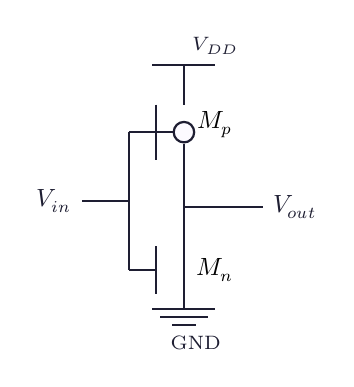
\begin{tikzpicture}[scale=1.0, thick, font=\small]
  % CMOS Schematic
  % pMOS
  \draw[line] (0, 1.8) -- (0, 1.3);
  \draw[draw=mydark, fill=hdrpurple!20] (0, 0.95) circle (0.13); % circle for pMOS gate
  \draw[line] (0, 0.8) -- (0, 0.3);
  \draw[line] (-0.7, 0.95) -- (-0.13, 0.95);
  \draw[line] (-0.35, 1.3) -- (-0.35, 0.6);
  \draw[line] (-0.35, 0.95) -- (-0.7, 0.95);
  \node at (0.4, 1.05) {$M_p$};

  % nMOS
  \draw[line] (0, -0.3) -- (0, -0.8);
  \draw[line] (0, -0.8) -- (0, -1.3);
  \draw[line] (-0.7, -0.8) -- (-0.35, -0.8);
  \draw[line] (-0.35, -0.5) -- (-0.35, -1.1);
  \node at (0.4, -0.8) {$M_n$};

  % Connections
  \draw[line] (-0.7, 0.95) -- (-0.7, -0.8);
  \draw[line] (-0.7, 0.075) -- (-1.3, 0.075) node[left] {$V_{in}$};
  \draw[line] (0, 0.3) -- (0, -0.3);
  \draw[line] (0, 0) -- (1.0, 0) node[right] {$V_{out}$};

  % Power Rails
  \draw[line] (-0.4, 1.8) -- (0.4, 1.8) node[above, font=\scriptsize] {$V_{DD}$};
  \draw[line] (-0.4, -1.3) -- (0.4, -1.3);
  \draw[line] (-0.3, -1.4) -- (0.3, -1.4);
  \draw[line] (-0.15, -1.5) -- (0.15, -1.5) node[below, font=\scriptsize] {GND};
\end{tikzpicture}
\end{tcolorbox}

\section{Voltage Transfer Characteristics (VTC)}

The VTC plot of $V_{out}$ vs. $V_{in}$ characterizes the inverter's static response.

\subsection{Five Regions of Operation}
The VTC curve is divided into 5 distinct regions based on the state of the two transistors:

\begin{tcolorbox}[tikzbox, title={CMOS Inverter Voltage Transfer Characteristics (VTC)}]
\centering
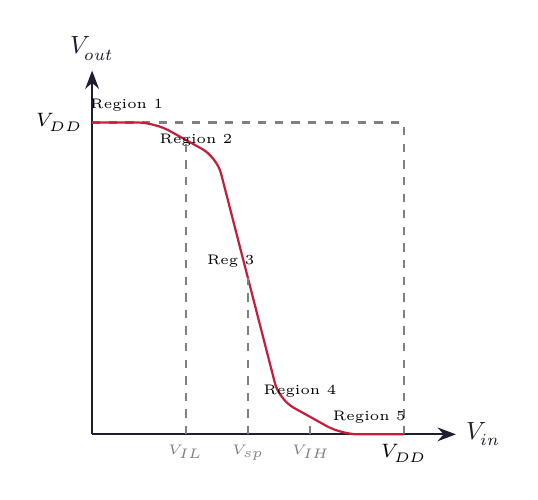
\begin{tikzpicture}[scale=1.1, thick, font=\small]
  % Axes
  \draw[arrow] (0, 0) -- (4.2, 0) node[right] {$V_{in}$};
  \draw[arrow] (0, 0) -- (0, 4.2) node[above] {$V_{out}$};
  
  % Limits
  \draw[dashed, gray] (3.6, 0) -- (3.6, 3.6);
  \draw[dashed, gray] (0, 3.6) -- (3.6, 3.6);
  \node[left, font=\scriptsize] at (0, 3.6) {$V_{DD}$};
  \node[below, font=\scriptsize] at (3.6, 0) {$V_{DD}$};

  % VTC Curve
  \draw[line, color=myred, rounded corners=6pt] (0, 3.6) -- (0.72, 3.6) -- (1.44, 3.2) -- (1.8, 1.8) -- (2.16, 0.4) -- (2.88, 0) -- (3.6, 0);

  % Regions labels
  \node[font=\tiny] at (0.4, 3.8) {Region 1};
  \node[font=\tiny] at (1.2, 3.4) {Region 2};
  \node[font=\tiny] at (1.6, 2.0) {Reg 3};
  \node[font=\tiny] at (2.4, 0.5) {Region 4};
  \node[font=\tiny] at (3.2, 0.2) {Region 5};

  % Critical Points (Slope = -1)
  % V_IL
  \draw[dashed, gray] (1.08, 0) node[below, font=\tiny] {$V_{IL}$} -- (1.08, 3.45);
  % V_IH
  \draw[dashed, gray] (2.52, 0) node[below, font=\tiny] {$V_{IH}$} -- (2.52, 0.15);
  % V_th (Switching Threshold)
  \draw[dashed, gray] (1.8, 0) node[below, font=\tiny] {$V_{sp}$} -- (1.8, 1.8);
\end{tikzpicture}
\end{tcolorbox}

\begin{enumerate}[label=\arabic*., leftmargin=*]
  \item \textbf{Region 1 ($0 \le V_{in} < V_{thn}$):} Input is low. nMOS is cut-off ($I_{Dn} = 0$). pMOS is ON in the linear region. $V_{out} = V_{DD}$.
  \item \textbf{Region 2 ($V_{thn} \le V_{in} < V_{sp}$):} nMOS turns ON in saturation ($V_{DSn} > V_{GSn} - V_{thn}$). pMOS is ON in linear region. $V_{out}$ begins to drop.
  \item \textbf{Region 3 ($V_{in} = V_{sp}$):} Switching threshold. Both nMOS and pMOS are in saturation. The output drops steeply.
  \item \textbf{Region 4 ($V_{sp} < V_{in} \le V_{DD} - |V_{thp}|$):} nMOS is ON in linear region. pMOS is ON in saturation region.
  \item \textbf{Region 5 ($V_{in} > V_{DD} - |V_{thp}|$):} Input is high. pMOS is cut-off ($I_{Dp} = 0$). nMOS is ON in linear region. $V_{out} = 0\,\text{V}$.
\end{enumerate}

\subsection{Derivation of Switching Threshold ($V_{sp}$)}
The switching threshold (or gate threshold voltage $V_{sp}$) is defined as the point where $V_{in} = V_{out}$. In Region 3, both transistors are in saturation:
\begin{equation}
  I_{Dn} = I_{Dp} \implies \frac{1}{2} k_n \left( V_{sp} - V_{thn} \right)^2 = \frac{1}{2} k_p \left( V_{DD} - V_{sp} - |V_{thp}| \right)^2
\end{equation}
Taking the square root on both sides:
\begin{equation}
  \sqrt{k_n} \left( V_{sp} - V_{thn} \right) = \sqrt{k_p} \left( V_{DD} - V_{sp} - |V_{thp}| \right)
\end{equation}
Divide by $\sqrt{k_n}$ and define the ratio $r = \sqrt{k_p / k_n}$:
\begin{equation}
  V_{sp} - V_{thn} = r \left( V_{DD} - V_{sp} - |V_{thp}| \right)
\end{equation}
\begin{equation}
  V_{sp} (1 + r) = V_{thn} + r \left( V_{DD} - |V_{thp}| \right)
\end{equation}
\begin{equation}
  V_{sp} = \frac{V_{thn} + r \left( V_{DD} - |V_{thp}| \right)}{1 + r}
\end{equation}
For a \textbf{symmetric inverter} where $k_n = k_p \implies r = 1$, and $V_{thn} = |V_{thp}|$:
\begin{equation}
  V_{sp} = \frac{V_{DD}}{2}
\end{equation}
To achieve a symmetric inverter ($k_n = k_p$), since electron mobility $\mu_n \approx 2.5\mu_p$, we must scale the channel widths:
\begin{equation}
  \mu_n C_{ox} \frac{W_n}{L_n} = \mu_p C_{ox} \frac{W_p}{L_p} \implies \left(\frac{W}{L}\right)_p \approx 2.5 \left(\frac{W}{L}\right)_n
\end{equation}

\subsection{Noise Margins ($NM_H, NM_L$)}
Noise margin measures the allowable electrical noise voltage on input terminals before the gate output state becomes corrupted.

\textbf{Critical Voltages}:
\begin{itemize}[leftmargin=*, itemsep=3.5pt]
  \item $V_{IL}$ (Input Low Voltage): The highest input voltage interpreted as Logic '0' (where $dV_{out}/dV_{in} = -1$).
  \item $V_{IH}$ (Input High Voltage): The lowest input voltage interpreted as Logic '1' (where $dV_{out}/dV_{in} = -1$).
  \item $V_{OL}$ (Output Low Voltage): Static low output: $V_{OL} = 0\,\text{V}$ for CMOS.
  \item $V_{OH}$ (Output High Voltage): Static high output: $V_{OH} = V_{DD}$ for CMOS.
\end{itemize}

\textbf{Formulas}:
\begin{equation}
  NM_L = V_{IL} - V_{OL} = V_{IL}
\end{equation}
\begin{equation}
  NM_H = V_{OH} - V_{IH} = V_{DD} - V_{IH}
\end{equation}

\section{Alternative load Inverters}

Before static CMOS was standardized, alternative single-channel (nMOS-only) designs were used to avoid fabricating pMOS devices.

\begin{itemize}[leftmargin=*, itemsep=3.5pt]
  \item \textbf{Resistive-Load Inverter:} Uses a passive resistor $R_L$ as the pull-up load. Drawbacks: consumes a massive silicon area for high resistance; has static power dissipation when output is low ($I_{static} = V_{DD}/R_L$).
  \item \textbf{Enhancement-Load Inverter:} Uses an enhancement-mode nMOS transistor as a load (gate connected to $V_{DD}$ or drain). Drawbacks: Output high voltage is degraded ($V_{OH} = V_{DD} - V_{thn}$), and suffers from static power dissipation when $V_{out}$ is low.
  \item \textbf{Depletion-Load Inverter:} Uses a depletion-mode nMOS transistor (with gate shorted to source, $V_{GS}=0$) as a load. Acts as a constant current source, yielding a sharper VTC transition and full logic swing ($V_{OH} = V_{DD}$), but still has high static power dissipation when output is low.
\end{itemize}

\begin{tcolorbox}[tikzbox, title={CMOS vs Depletion-Load Inverter Comparison}]
\renewcommand{\arraystretch}{1.4}
\par\noindent
\begin{tabularx}{\linewidth}{|B{3.2cm}|Y|Y|}
\hline
\textbf{Feature} & \textbf{\color{myred}Static CMOS Inverter} & \textbf{\color{myteal}Depletion-Load Inverter} \\
\hline
\textbf{Device Count} & 2 (1 nMOS, 1 pMOS). & 2 (1 enhancement, 1 depletion nMOS). \\
\hline
\textbf{Logic Swing} & Full rail-to-rail swing ($0$ to $V_{DD}$). & High swing (nearly $0$ to $V_{DD}$). \\
\hline
\textbf{Static Power} & Zero (ignoring tiny leakage). & High (when $V_{out}$ is low). \\
\hline
\textbf{Transition Width} & Narrow, sharp drop. & Moderate. \\
\hline
\textbf{Fabrication} & High complexity (well formation). & Low complexity (single-channel). \\
\hline
\end{tabularx}
\tcbset{colbacktitle=mypurple, coltitle=white}
\end{tcolorbox}

\newpage
% ===============================================================================
% MANDATORY QUICK REVISION PAGE
% ===============================================================================
\begin{center}
  {\large\bfseries\color{myred} Quick Revision --- Module 4}\\[3pt]
  {\small\color{mydark} MOS \& CMOS Inverters (Static Characteristics) $|$ PE-EC603C}
\end{center}
\noindent{\color{myred}\rule{\linewidth}{1.2pt}}
\vspace{4pt}

\begin{tcolorbox}[formulabox, title={\textbf{Key Inverter Equations}}]
$$V_{sp} = \frac{V_{thn} + r(V_{DD} - |V_{thp}|)}{1 + r} \qquad \text{where} \ r = \sqrt{\frac{k_p}{k_n}} = \sqrt{\frac{\mu_p W_p L_n}{\mu_n W_n L_p}}$$
$$\text{Symmetric Inverter Width Ratio:} \quad \left(\frac{W}{L}\right)_p \approx 2.5 \left(\frac{W}{L}\right)_n \qquad V_{sp} = \frac{V_{DD}}{2}$$
$$NM_L = V_{IL} - V_{OL} = V_{IL} \qquad NM_H = V_{OH} - V_{IH} = V_{DD} - V_{IH}$$
\end{tcolorbox}

\begin{tcolorbox}[defbox, title={\textbf{One-Line Definitions}}]
\begin{itemize}[leftmargin=*, itemsep=2.5pt, topsep=0pt]
  \item \textbf{VTC:} Plot of output voltage against input voltage characterizing static gain and noise immunities.
  \item \textbf{Switching Threshold ($V_{sp}$):} Input voltage at which the output voltage equals the input voltage ($V_{in} = V_{out}$).
  \item \textbf{Noise Margin:} The maximum noise voltage that can be added to the input signal without corrupting the output logic state.
  \item \textbf{Symmetric Inverter:} An inverter with identical pull-up and pull-down strengths, placing $V_{sp}$ exactly at $V_{DD}/2$.
  \item \textbf{Static Power Dissipation:} Power consumed by the gate when inputs are static (non-switching).
  \item \textbf{Depletion Load:} An nMOS transistor with $V_{th} < 0$, configured with gate shorted to source to act as a current source.
\end{itemize}
\end{tcolorbox}

\begin{tcolorbox}[exambox, title={\textbf{Frequently Asked / Viva Questions}}]
\begin{enumerate}[topsep=0pt, label=\textbf{Q\arabic*.}, itemsep=5pt]
  \item \Q{Why is the static power dissipation of a CMOS inverter practically zero?}
    Because in either steady state (Input = '0' or Input = '1'), one of the two series transistors (either pMOS or nMOS) is completely cut off, presenting an open circuit. Consequently, no direct path exists from $V_{DD}$ to GND, and current flow is limited to subthreshold and junction leakages (picoamps).
  \item \Q{Derive the switching threshold $V_{sp}$ of a CMOS inverter.}
    Equating saturation currents $I_{Dn} = I_{Dp} \implies \frac{1}{2} k_n (V_{sp} - V_{thn})^2 = \frac{1}{2} k_p (V_{DD} - V_{sp} - |V_{thp}|)^2$. Taking the square root, collecting terms, and solving for $V_{sp}$ yields $V_{sp} = \frac{V_{thn} + r(V_{DD} - |V_{thp}|)}{1+r}$ where $r = \sqrt{k_p/k_n}$.
  \item \Q{How do we design a symmetric CMOS inverter and why is it preferred?}
    A symmetric inverter has $V_{sp} = V_{DD}/2$, which maximizes both noise margins ($NM_L = NM_H$) and balances rise and fall propagation delays. It is achieved by setting $k_n = k_p \implies \mu_n(W/L)_n = \mu_p(W/L)_p \implies (W/L)_p \approx 2.5(W/L)_n$.
  \item \Q{Define Noise Margin and write its formulas for a CMOS inverter.}
    Noise margin represents the gate's noise immunity. For CMOS, since $V_{OL}=0$ and $V_{OH}=V_{DD}$, the margins are $NM_L = V_{IL} - V_{OL} = V_{IL}$ and $NM_H = V_{OH} - V_{IH} = V_{DD} - V_{IH}$, where $V_{IL}$ and $V_{IH}$ are input voltages where the VTC slope $dV_{out}/dV_{in} = -1$.
  \item \Q{Explain the VTC region 3 of a CMOS inverter.}
    In Region 3, the input is close to $V_{DD}/2$. Both nMOS and pMOS are in saturation simultaneously, acting as high-impedance current sources. This creates a very high voltage gain ($dV_{out}/dV_{in} \ll -1$), causing a steep drop in $V_{out}$.
  \item \Q{What are the disadvantages of a resistive-load inverter?}
    First, it consumes static power ($P = V_{DD}^2/R_L$) whenever the output is low because the pull-down nMOS is ON. Second, to get low $V_{OL}$, $R_L$ must be very large (tens of $\text{k}\Omega$), which requires a massive surface area on silicon compared to a transistor.
  \item \Q{Why does an enhancement-load inverter suffer from degraded $V_{OH}$?}
    In an enhancement-load nMOS inverter, the load transistor turns OFF when the output rises to $V_{DD} - V_{thn}$ because its gate-source voltage drops below the threshold voltage. Thus, it cannot pull the output all the way up to $V_{DD}$.
  \item \Q{Explain the depletion-load inverter and its advantage over resistive-load.}
    The depletion-load inverter uses a depletion-mode nMOS with $V_{th} < 0$ and gate shorted to source ($V_{GS}=0$). It behaves as a constant current source rather than a passive resistor, which pulls the output up to the full $V_{DD}$ and yields a sharper VTC transition.
  \item \Q{If a CMOS inverter has $V_{DD} = 3.3\,\text{V}$, $V_{thn} = 0.7\,\text{V}$, $|V_{thp}| = 0.8\,\text{V}$, and $r = 1.0$, calculate $V_{sp}$.}\\
    Using the formula: $V_{sp} = \frac{V_{thn} + r(V_{DD} - |V_{thp}|)}{1+r} = \frac{0.7 + 1.0 \times (3.3 - 0.8)}{1 + 1} = \frac{0.7 + 2.5}{2} = 1.6\,\text{V}$.
  \item \Q{How does noise margin scale when we reduce the supply voltage $V_{DD}$?}
    As $V_{DD}$ scales down, the total transition range of the VTC shrinks. Since critical points $V_{IL}$ and $V_{IH}$ scale proportionally with $V_{DD}$, the absolute noise margins ($NM_L, NM_H$) decrease, making the circuit more sensitive to external electrical noise.
\end{enumerate}
\end{tcolorbox}

\end{document}
